%\chapter{User Interface}
%\label{ch:ui}
 
All the previous work becomes irrelevant without adding a way for the user to interact with the system. This section describes the work that went into the creation of the frontend application to support the 15-Minute city concept.

\subsection{Implementations}
\label{ss:ui-implementations}

Web requirements keep changing, with developers having to support dozens of different browsers, devices, and resolutions. Enter the frontend frameworks, a solution ready to deal with all these problems, on top of it, it also implements multiple functions such as routing, saving development time by not having to reinvent the wheel. In the following sections, we will analyse some of the most popular tools currently available in the market, and how they fare against each other.

\subsubsection{Angular}
\label{sss:angular}

Angular is a component based framework that follows a tree structure, where there is a root with an infinite possibility of children and sibling components. Parents can communicate with children by binding information to them, but a child is unaware of the origin of the data, if it wishes to communicate with the parent, an event has to be emitted. This structure makes components reusable and self-contained.

Components are classes annotated with \textbf{@Component}, and consist of three separate files: .ts, .css and .html. Each component provides a series of life cycle hooks, as seen in the transitions in Fig. \ref{fig:angular-lifecycle}.

\begin{figure}[H]
	\centering
	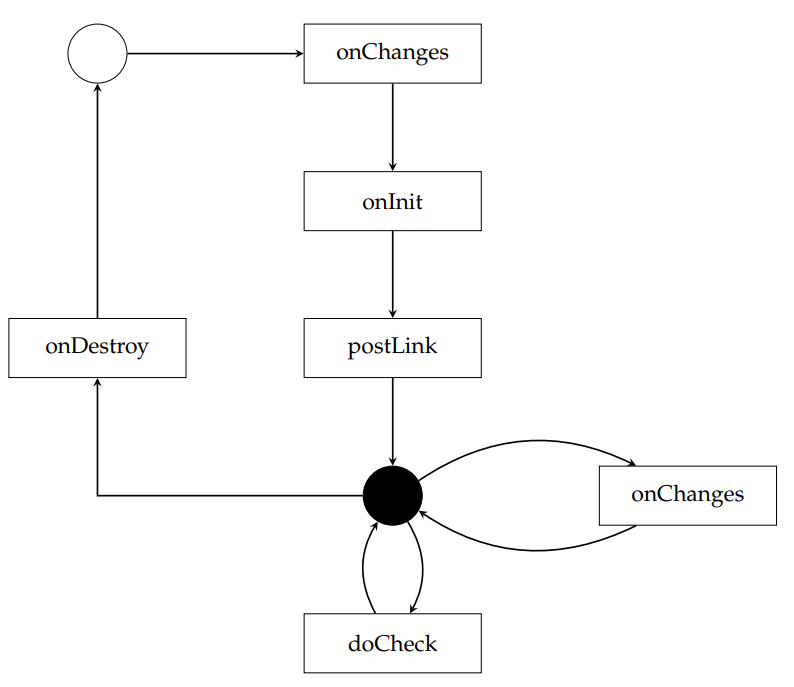
\includegraphics[width=0.75\linewidth]{Chapters/img/frontend/angular-lifecycle.png}
	\caption{Angular life-cycle \cite{react-lifecycle}}
	\label{fig:angular-lifecycle}
\end{figure}

\begin{itemize}
    \item \textbf{onInit} is executed once per component upon creation of the component. It is meant to be used for initial setup and registration of further event handlers.
    \item \textbf{onChanges} is a callback executed whenever a one-way bound variable is updated. It typically occurs during two different stages of the life cycle. Initially, upon creation of the component when initial values for the variables are passed to the component, the method is executed even before the \textit{init} callback. The second time, and which may occur multiple times, is during the lifespan of the component. Whenever a binding is updated, the \textit{onChanges} callback is called with a reference to the variable;
    \item \textbf{doCheck} is called whenever the internal change detection cycle of AngularJS is executed. It provides the possibility to implement custom change detection procedures.
    \item \textbf{onDestroy} called when the component becomes detached from the DOM and the corresponding scope is destroyed
    \item \textbf{postLink} called after the initial setup has been completed and the DOM is constructed. Access to children elements is still restricted, due to asynchronous template loading of child elements in AngularJS.
\end{itemize}

Angular also uses Service, a class with a narrow and well-defined purposed, which angular distinguishes from components to increase modularity and reusability. By separating a component's view-related functionality from other kinds of processing, component classes can remain lean and efficient. A component can delegate certain tasks to services, such as fetching data from the serer, validating user input, etc...  By defining such processing tasks in an injectable service class, it makes those tasks available to any component.

This idea of injecting service classes comes from the concept of \acrfull{di}, a design pattern in which a class requests dependencies from external sources rather than creating them. In Angular, components consume services; that is, a service can be injected into a component, giving the component access to that service class. In angular, services are annotated with \textbf{@Injectable()}.


\subsubsection{React}
\label{sss:react}

\todo[inline]{Decidimos deixar este capitulo para o fim, vamos tentar entender mais tarde se faz sentido manter aqui ou no SotA. A dúvida está em que apesar de ser sobre react, está muito relacionada com padrões de desenho de software.

Possivel solução: mudar nome de react para 'design patterns', elaborar as secções de MVC, MVVM e manter o Flux. Passar as informacoes do react em si, para a implementacao.}


%% -- Created: 07-07-21
%% -- Last edit: 07-07-21

React \footnote{\url{https://reactjs.org/}} is a Javascript library used to build \acrshort{ui}s, it can be used in isolated parts or to create \acrshort{ui}s for whole web applications. React focus entirely on the creation of Views, as such it does not enforce any architecture pattern.

React relies on composition to build complex \acrshort{ui}s from small building blocks called \textbf{components}~\cite{react-lifecycle-functions}. Components consist of a render method that returns a description of what to render, which  can either be HTML or other react components. The description of what to render uses a syntax called \acrlong{jsx} (\acrshort{jsx}) which is a combination of HTML and Javascript. 


React applications have two essential building blocks \textbf{state} and \textbf{props}. State allows components to "remember" things, but it can also be altered based on user interaction or other actions within the application~\cite{react-state-and-lifecycle}. State is not mandatory, and components with it are called stateful components while states without it are called presentation components.

Props, or properties, are immutable data passed onto a component upon construction. This is what makes React components flexible and reusable, as one component can behave and look differently depending on the props passed to it.

In React, data flows downwards through the component tree using props. For a child component to interact with its parent, callback functions are passed as props. In large applications this is not ideal since it can lead to deep trees, which forces data and callback functions to pass through multiple levels. This process is referred to as "\textbf{props-drilling}" and makes the components tightly coupled and less maintainable.

Each component can be defined as a \textbf{class-based} or \textbf{function} component. A class-based component is created by extending the \textit{React.Component}. The state of this type of components is updated using the method \textit{setState()} and read by using \textit{this.state} within the class. Using the setState() method makes the component re-render which is not the case when mutating the state directly. Class-based components include \textbf{life-cycle} methods that can be used to create more complex behaviour.

This life-cycle methods~\cite{react-state-and-lifecycle} are built-in methods called when a state or prop updates, before or after a component has rendered or when a component is destroyed, as shown in Fig. \ref{fig:react-lifecycle}.

\begin{figure}[H]
	\centering
	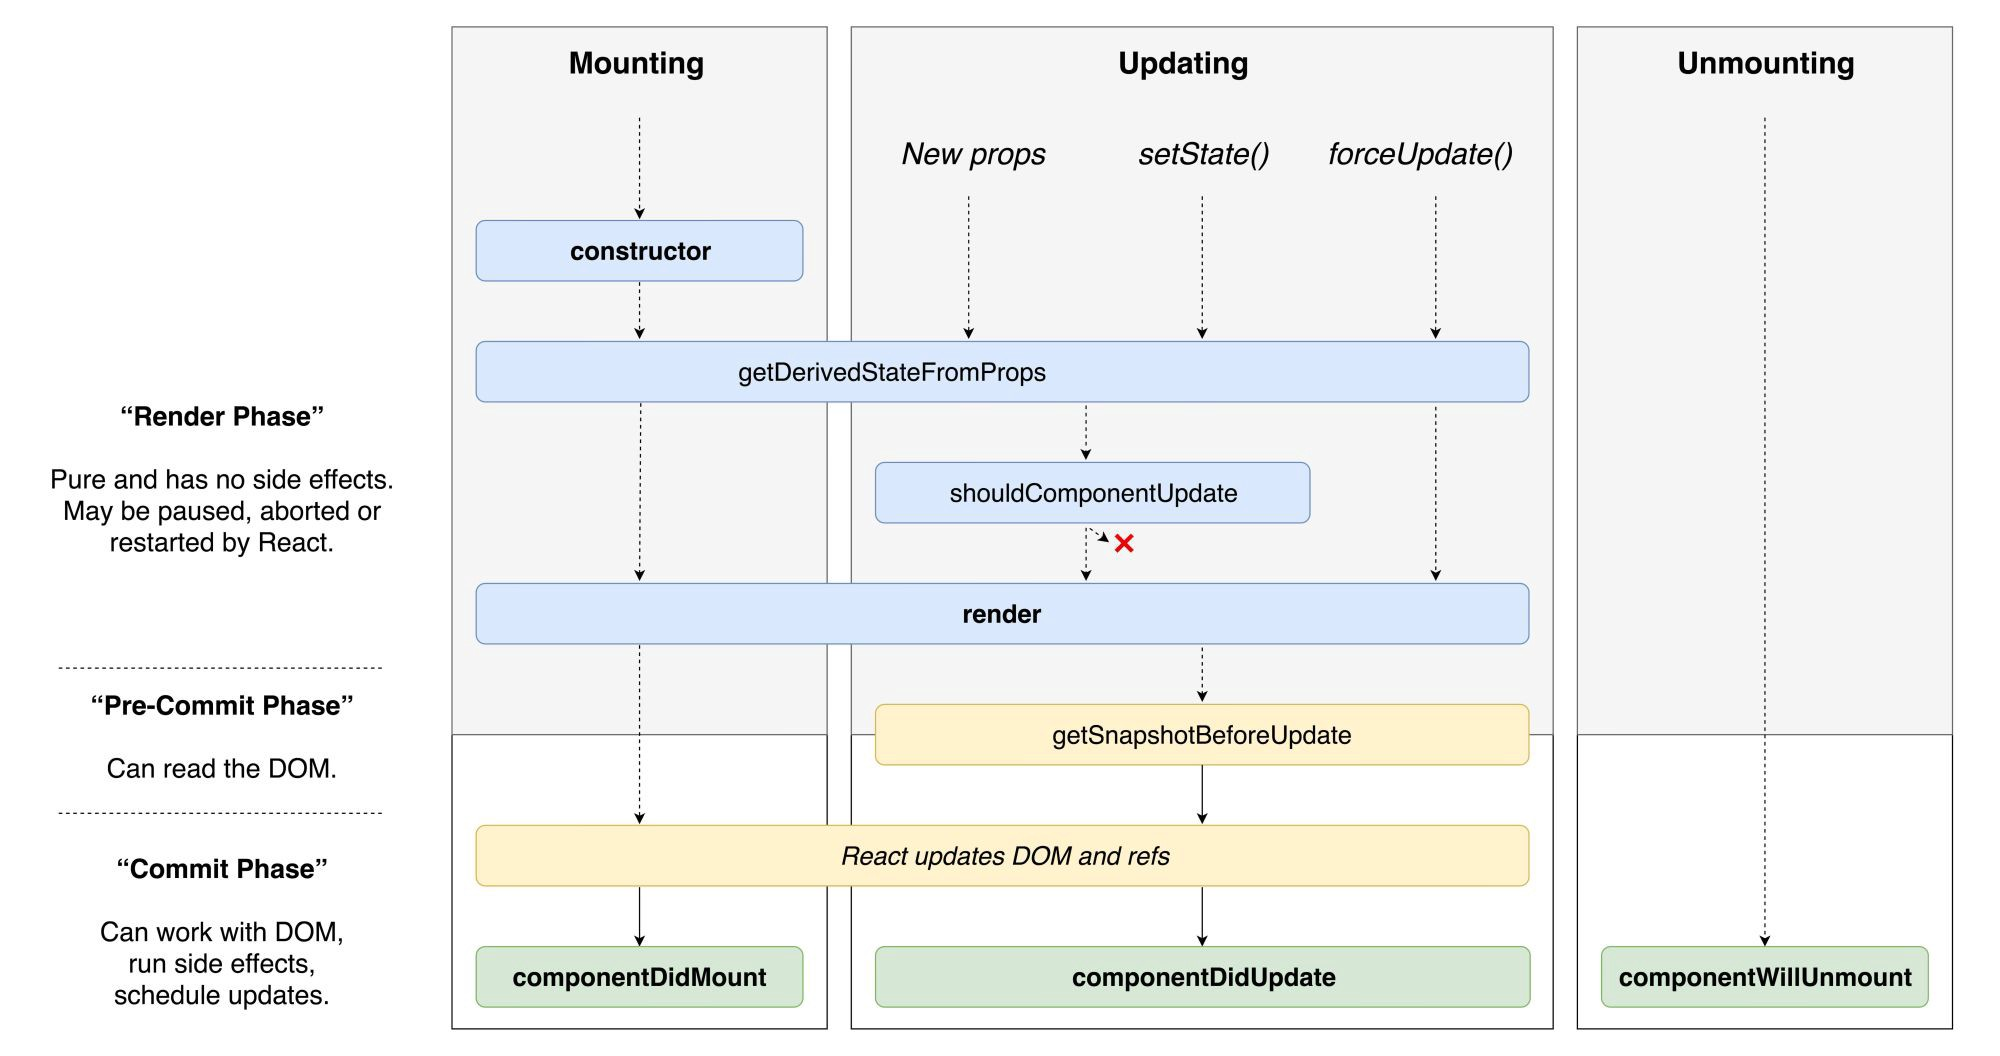
\includegraphics[width=1\linewidth]{Chapters/img/2_background/react-lifecycle.jpeg}
	\caption{React life-cycle \cite{react-lifecycle}}
	\label{fig:react-lifecycle}
\end{figure}

This cycle is split into three phases: \begin{inparaenum}[1)] \item \textbf{mounting}, the birth of the component; \item \textbf{updating}, growth of the component; \item \textbf{unmounting}, the dead of the component \end{inparaenum}. Here's an overview of the most commonly used methods~\cite{react-lifecycle-functions}:

\begin{itemize}
    \item \textbf{render} is the most used. Handles the rendering of components. It is a pure function (no side-effects and always returns the same output with the same inputs) and as such, it should not be used to set the state;
    
    \item \textbf{componentDidMount} is called as soon as the component is mounted and ready. Used to initiate \acrshort{api} calls, if data from a remote endpoint is needed. Updating state here will cause another rendering but it will happen before the browser updates the \acrshort{ui} (to ensure that the user will not see any \acrshort{ui} updates with double rendering).
    
    \item \textbf{componentDidUpdate} happens as soon as the updating happens, its mostly used for updating \acrshort{dom} in response to prop or state changes. State updates here must be done with caution to avoid infinite update loops.
    
    \item \textbf{componentWillUnmount} happens before the component unmounts and is destroyed. Used for data cleanup.
\end{itemize}

Function components are pure functions that accept props as input and return a \acrshort{jsx} element. To given them access to state and life-cycle methods as class-based components, \textbf{React hooks} are used. By combining component functions with hooks, the size and complexity of an application in comparison to class-based components is reduced.

Hooks~\cite{react-hooks} are used for more advanced function components and can also be customized, which promotes re usability of functionality between components. They follow a naming convention starting with the word "use", as can be seen while looking at three of the main hooks:

\begin{itemize}
    \item \textbf{useState} As state does not exists in function components by default, useState is used which preserves the state throughout the lifetime of the component. This hook, and all others, can be used more than once inside the same component;
    \item \textbf{useEffect} allows for the replacement of life-cycle mthods. This hook will execute a function for every rerender of the component by default, but can also be customized to only execute for certain changes;
    \item \textbf{useContext} allows data to be shared between components in the component tree without requiring props-drilling. Data is added to the Context and made available through a \textbf{Provider}.
\end{itemize}

%since State does not exist in a component by default, instead they use a React hook named \textit{\textbf{useState}} which preserves the state throughout the lifetime of the component. This hook, and all others, can be used more than once inside the same component.

%Since life-cycle methods do not exist in function components, they had to be recreated using the \textit{\textbf{useEffect}} hook, which will execute a function for every rerender of the component by default but can be customized to only execute for certain changes.

%Another hook is the \textbf{\textit{useContext}} hook which allows data to be shared between components in the component tree without using props-drilling. Data is added to the Context and made available through a \textbf{Provider}.

The provider takes one property named value where the data for the Context is specified which can be variables, functions, or objects. By wrapping children components inside the Provider component, the Context data can be accessed from any child component using a Consumer available to the Context instance as well. Worth noting that the application is not limited to one context.

\subsection{Flux - Architectural Pattern}
\label{ss:flux}

%% -- Created: 07-07-21
%% -- Last edit: 07-07-21

Since React does not enforce architectural patterns all functionality for a web application could, in theory, be placed in a single module that would handle everything from data fetching to business logic. But that leads to an error-prone application that would be hard to maintain, therefore architectural patterns are necessary to build well-structured high-quality applications.

As React applications have an unidirectional data flow, as described before, each component has its own data stored in its state. For larger React applications, more advanced architectural patterns are needed to make the application maintainable, such as \textbf{Flux} \footnote{\url{https://facebook.github.io/flux/}}.

The flux architectural pattern was invented by Facebook, it was derived from the \acrlong{mvc} (\acrshort{mvc}) pattern (Fig. \ref{fig:mvc-pattern}) with the purpose of having more control of the data flow of the application. The problem of using \acrshort{mvc} was the lack of control when updating Models and Views, since the communication between them is bidirectional, it means the Model can update the View while the View also can grab data from the model and update it itself. It becomes hard to maintain and test, as it is difficult to predict what the state of the View has become because changes can come from different sources. 

\begin{figure}[H]
     \centering
     \begin{subfigure}[b]{0.49\textwidth}
         \centering
         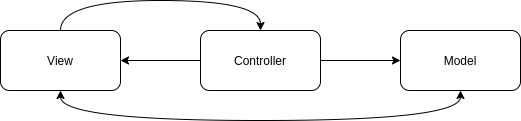
\includegraphics[width=\textwidth]{Chapters/img/2_background/mvc-pattern.jpg}
         \caption{MVC Pattern}
         \label{fig:mvc-pattern}
     \end{subfigure}
     \hfill
     \begin{subfigure}[b]{0.49\textwidth}
         \centering
         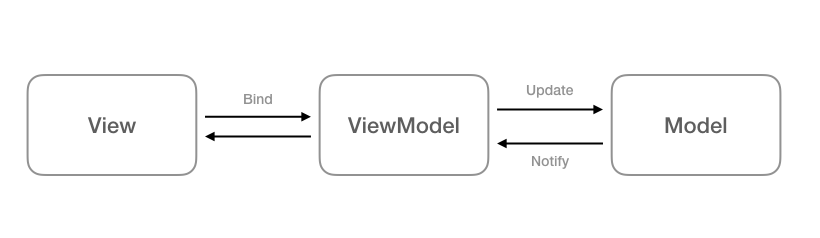
\includegraphics[width=\textwidth]{Chapters/img/2_background/mvvm-pattern.png}
         \caption{MVVM Pattern~\cite{mvvm-pattern-figure}}
         \label{fig:mvvm-pattern}
     \end{subfigure}
     \caption{Base architectural patterns}
\end{figure}

\acrlong{mvvm} (\acrshort{mvvm}) (Fig. \ref{fig:mvvm-pattern}) tried to solve this problem by tightly coupling views to a related ViewModel by having a two-way data binding for getting and setting values~\cite{mvvm-problems}. The ViewModel manages the Model data and the associated view using data bindings rather than through events, which makes it more predicable and easier to test.

At Facebook, models providing data to different views, views updating Models based on user interaction and Models updating other Models data, led to problems debugging the data flow when developing web applications~\cite{facebook-debugging-problems}. Flux suggests a solution to this by using an unidirectional data flow.

\begin{figure}[H]
	\centering
	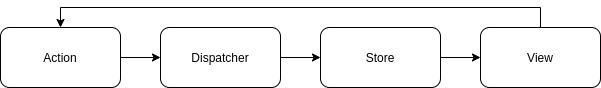
\includegraphics[width=1\linewidth]{Chapters/img/2_background/flux-pattern.jpg}
	\caption{Flux pattern}
	\label{fig:flux-pattern}
\end{figure}

The pattern consists of four elements:

\begin{itemize}
    \item \textbf{Stores} are where all the data in the application is located, only them can manipulate it. Information is exposed through public getters for views;
    \item \textbf{Views} can subscribe to stores and update accordingly. It is different from the MVC patterns where Views can update the data in the model freely;
    \item \textbf{Actions} are used to update data in the store. One Actions exists for every change needed in the application, it can happen due to a user interaction or a network request. Each Action is an object containing two fields: a \textbf{type} and a \textbf{payload}. The type is a unique string describing the action (e.g., ADD\_ESTATE). The payload field containers the data to update the Store. For an Action to reach a Store it goes through the Dispatcher;
    \item \textbf{Dispatcher} is responsible for handling incoming actions before passing them to the Store and deciding in which order the actions should be dispatched. By using actions, the operations are decoupled from the Views and can be reused for multiple Views.
\end{itemize}

\subsubsection{Vue}
\label{sss:vue}

Vue is a popular JavaScript framework that shares many similarities with React, it was created as a lightweight alternative to Angular and as such as many similar features but with less extra concepts. The core library of Vue focuses exclusively on the view layer and can be integrated with other libraries and projects, while also supporting complex \acrfull{spa}.

It uses an HTML based template syntax, it has a characteristic signature of declaring syntax using a "v-" prefix, which is its way of identifying Vue-specific attributes. An example of this are the two most used commands in Vue \textit{v-bind} and \textit{v-on}, which are used to bind data and to listen to events, respectively.

\subsection{Comparing frameworks}

All these frameworks have in common a component-based structure, by splitting the application into various independent parts, it allows developers to work on each individual function of the application asynchronously, thus leading to a more flexible development process, maintaining the same ideology we gained from the microservices.

Vue and React both use a virtual DOM, with VUE it consists of multiple virtual nodes that manage what information should be displayed and interacts with the real DOM to update the data on the HTML page, on the other hand React uses the virtual DOM to handle many of the rendering tasks using as little DOM manipulation as possible, thus decreasing the time and resources needed for updates. In contrast, Angular does not use a virtual DOM, instead it converts components into classes that can be displayed onto the DOM.

What sets React apart from the other frameworks is that React is only a UI library rather than a full-fledged Javascript framework like the other two. Which may seem like an disadvantage due to having less features, but actually makes it an optimal tool when the emphasis is on the interface.

For this reason, React was the winner library for this project due to its simplicity and freedom, which allowed us to focus on creating interfaces.

\subsection{Solution}
\label{ss:ui-solution}

The following sections describe the implementation details of the main features present in the frontend, created in React. Including some of the advantages of working with components, and how have we created our code to follow the flux design pattern. It is split into two main sections, the \textbf{user} and \textbf{zones}.

\subsubsection{User}
\label{s:user}

To register and authenticate users, we had to create multiple supporting pages. All these pages are mostly composed of simple forms, to assist with the validation and error handling we opted to use \textbf{Formik~\url{https://formik.org/}}, simplifying the creation process. 

\begin{figure}[H]
     \centering
     \begin{subfigure}[b]{0.49\textwidth}
         \centering
         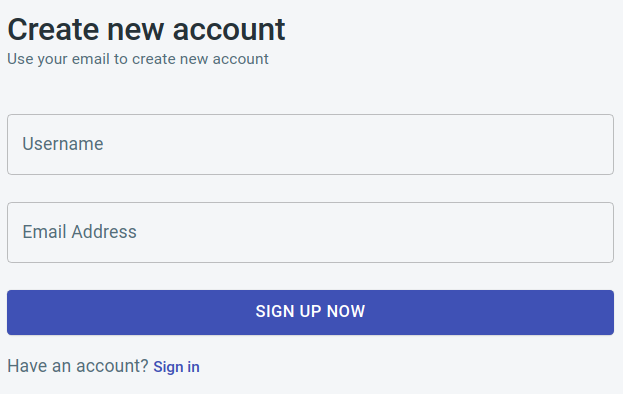
\includegraphics[width=0.8\linewidth]{Chapters/img/frontend/signUp.png}
    	\caption{Sign up}
    	\label{fig:signup}
     \end{subfigure}
     \hfill
     \begin{subfigure}[b]{0.49\textwidth}
         \centering
         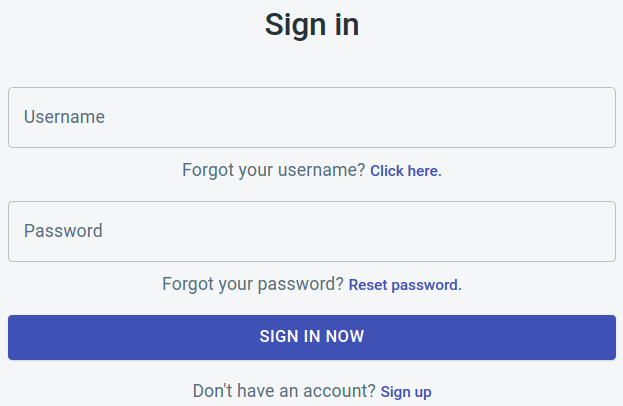
\includegraphics[width=0.8\linewidth]{Chapters/img/frontend/login.png}
	\caption{Sign in}
	\label{fig:signin}
     \end{subfigure}
     \caption{Registering and Authentication}
\end{figure}

\begin{figure}[H]
    \centering
    \begin{subfigure}[b]{0.49\textwidth}
        \centering
        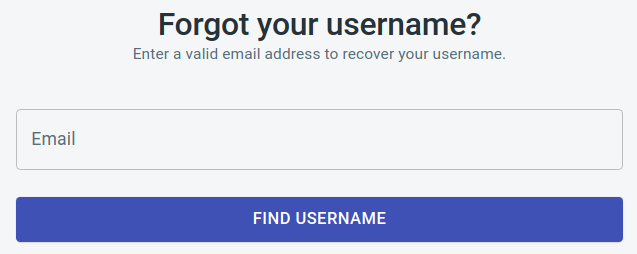
\includegraphics[width=0.8\linewidth]{Chapters/img/frontend/forgotUsername.png}
        \caption{Forgot username}
        \label{fig:forgotUsername}
     \end{subfigure}
     \hfill
     \begin{subfigure}[b]{0.49\textwidth}
        \centering
        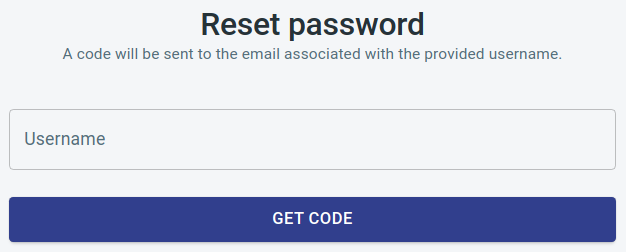
\includegraphics[width=0.8\linewidth]{Chapters/img/frontend/resetPassword.png}
        \caption{Reset password}
        \label{fig:resetPassword}
     \end{subfigure}
     \caption{Recovery}
\end{figure}

Upon creating an account, the user is prompted to fill out his profile. These components were designed in a way that would follow the \textbf{flux pattern} mentioned previously, which helps with the separation of concerns (rendering and state management). React provides the \textbf{useReducer()} hook that does so by extracting the state management out of the component. 

To understand the useReducer() hook it is necessary to first understand the following concepts:

\begin{itemize}
    \item \textbf{Initial State} is the value that the state is initialized with;
    \item \textbf{Action} is an object that describes how to update the state;
    \item \textbf{Dispatch} is a function that sends an action object;
    \item \textbf{Reducer} is a function that accepts 2 arguments, current state and an action. Based on the action, it must update the state in an immutable manner and return the new state.
\end{itemize}

\begin{figure}[h]
	\centering
	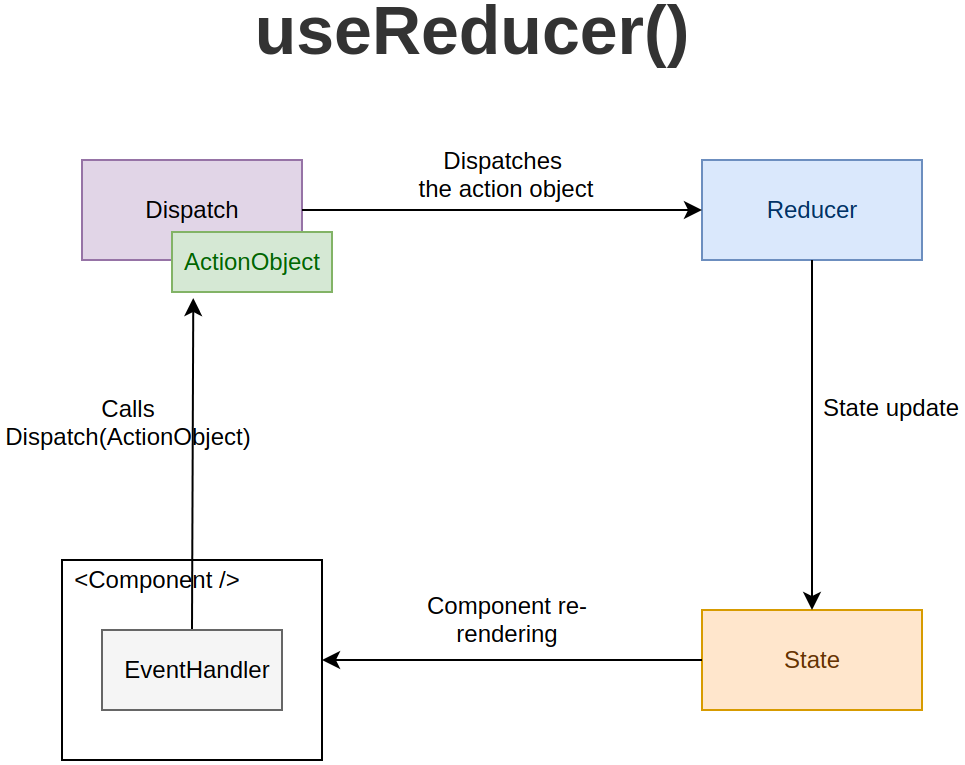
\includegraphics[width=0.5\linewidth]{Chapters/img/frontend/useReducer.png}
	\caption{useReducer() flow details~\cite{react-use-reducer}}
	\label{fig:useReducer}
\end{figure}

The diagram in Figure \ref{fig:useReducer} demonstrates the events that occur while using the useReducer() hook. Using the chip component (Fig. \ref{fig:ui-stepper-2}), used during the profile creation (Fig. \ref{fig:profile-stepper}). We start by capturing \textit{onClick()} events in the component, which are used to call the dispatch with an action to perform. In the following Listing (\ref{lst:dispatch}), the \textbf{ADD\_SELECTED\_FEATURE} was sent to the reducer.

%\begin{lstlisting}[language=Java, caption={EventHandler dispatching actions}, position={bottom}, label={lst:dispatch}]
\begin{lstlisting}[language=Java, caption={EventHandler dispatching actions}, label={lst:dispatch}]
const [state, dispatch] = useContext(FeaturesChipsContext);

const handleClick = (feature) => {

    if(state.selectedFeatures.length < MAX_FEATURES || feature.color == 'primary'){
        if(feature.color == 'default'){
            dispatch({
                type: "ADD_SELECTED_FEATURE",
                payload: {
                    feature: feature
                }
            });
        }
    ...
\end{lstlisting}

The reducer is implemented as a switch that updates the state according to the performed action, which for this action, alters the state by adding a new value to the selected feature list.

%\begin{lstlisting}[language=Java, caption={Reducer processing actions}, position={bottom}, label={lst:reducer}]
\begin{lstlisting}[language=Java, caption={Reducer processing actions}, label={lst:reducer}]
const [state, dispatch] = useReducer(reducer, initialState);

const reducer = (state, action) => {

    switch (action.type) {
        case "UPDATE_CHIPS":
            return {
                chips: action.payload.features
            };
        case "ADD_SELECTED_FEATURE":
            return {
                ...state,
                selectedFeatures: [...state.selectedFeatures, action.payload.feature.value]
            };
    ...
\end{lstlisting}

All the steps during the profile creation follow the same pattern. Taking advantage of having everything split into components, the same components are then reused in the preferences tab, where the user is allowed to update his preferences.

\begin{figure}[h]
	\centering
	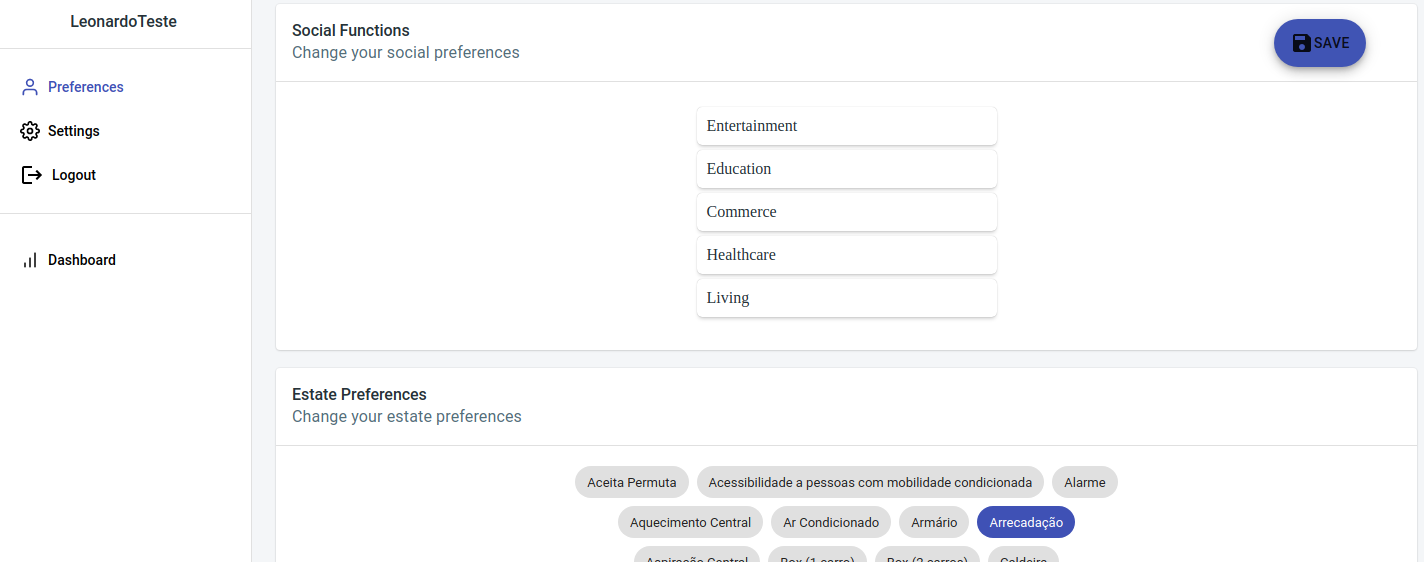
\includegraphics[width=0.6\linewidth]{Chapters/img/frontend/UserPreferences.png}
	\caption{Update user preferences}
	\label{fig:userPreferences}
\end{figure}

The same happens in the settings tabs, where the component used during the recovery process is used once again to change the password in a different context.

\begin{figure}[h]
	\centering
	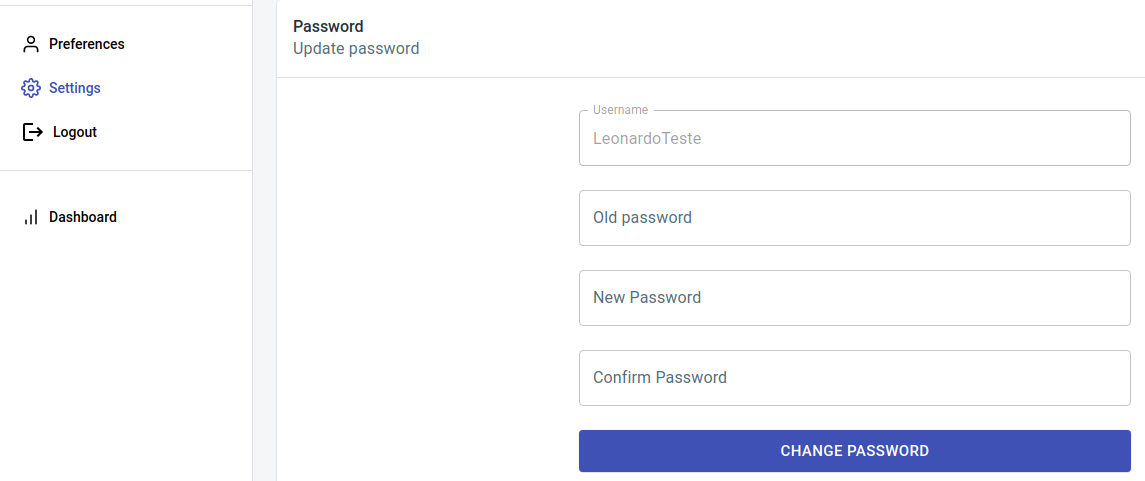
\includegraphics[width=0.6\linewidth]{Chapters/img/frontend/UserSettings.png}
	\caption{Update user settings}
	\label{fig:userSettings}
\end{figure}


\subsubsection{Dashboard} 
\label{sss:dashboard}

The dashboard is the main page of the application, when the user picks a new location to analyse, he is redirected to the dashboard. In the previous sections, while detailing the logic within the backend, it was shown how it looked (Figure \ref{fig:overviewDashboard}), now we will detail how each row was actually implemented in the frontend.

\paragraph{Zone overview} highlights some of the data gathered about the city such as the price and estate size. Most of the work for these information is done in the backend, and as such, there's nothing to highlight.

\begin{figure}[h]
	\centering
	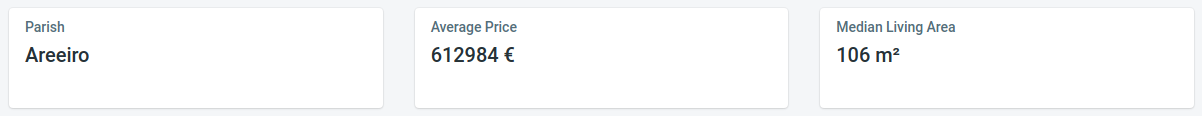
\includegraphics[width=1\linewidth]{Chapters/img/frontend/OverviewHeader.png}
	\caption{Random trivia about the selected zone}
	\label{fig:overviewHeader}
\end{figure}

\paragraph{Map} displays to the user several layers of geographical information composed of: \textbf{Points of Interest}, \textbf{Estates} and the \textbf{Zone}. It is built out of two different pieces, the header which includes multiple togglable buttons that allow the user to display only the relevant \acrshort{poi} and the map itself. As they both need to communicate, it was required to apply a technique known as \textit{Lifting State Up}, where a parent component was created to house both children, this way the parent is responsible for managing the estate of both subcomponents.

\begin{figure}[h]
	\centering
	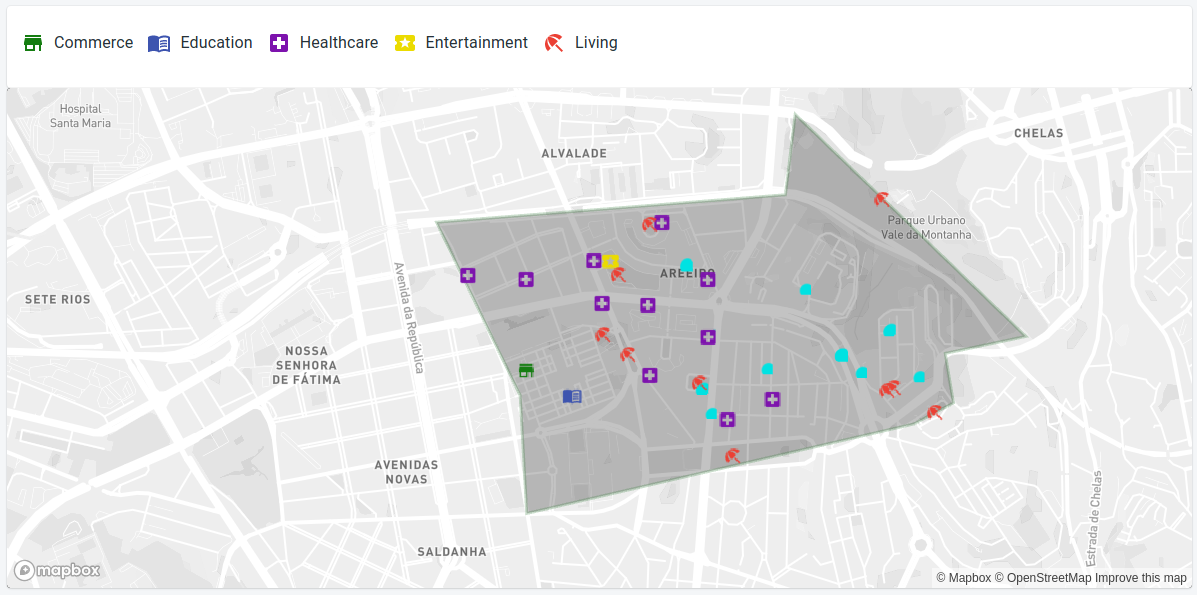
\includegraphics[width=1\linewidth]{Chapters/img/frontend/OverviewMap.png}
	\caption{Map}
	\label{fig:overviewMap}
\end{figure}

To control the state, the parent sends a callback function to the child component (handleCategoriesChange), allowing the map management component to handle the \textit{onClick()} events received within each button.

%\begin{lstlisting}[language=Java, caption={MapManagement component}, position={bottom}, label={lst:mapManagement}]
\begin{lstlisting}[language=Java, caption={MapManagement component},  label={lst:mapManagement}]
const handleCategoriesChange = (event) => {
    setState({ ...state, [event.target.name]: event.target.checked });
};

return <Grid item xs={12} width={'50%'} height={'50%'} >     
    <MapHeader onCategoriesChange={handleCategoriesChange} state={state}/>
     
    <Card style={{position: 'relative', background: 'black', minHeight:'500px'}}>
        <CardContent>
            <MapOSRM  locationId={localStorage.getItem('locationId')} locationType={props.zone.type} categories={getCatIds()}/>

            {/* <MapCluster /> */}
        </CardContent>
    </Card>
</Grid>
\end{lstlisting}

With the state handled by the manager component, it can be sent to the map component which can now render the selected social functions. To visualize the geospatial data we chose \textbf{deck.gl~\footnote{\url{https://deck.gl/}}} an open source geospatial analysis toolbox built by Uber on top of the Mapbox GL JS library, it is built to visualize massive datasets without compromising performance (e.g., Uber hundreds of millions of trips). For the application use-case, their layered approach to data visualization turned out to be extremely valuable, allowing us to render all of our three layers of data separately and improve the user experience as the user is presented some of the data while the rest is rendering.

%\begin{lstlisting}[language=Java, caption={Example of a GeoJSON layer, used to represent the zone geometry as seen in Fig. \ref{fig:overviewMap}}, label={lst:mapLayer}, position={bottom}]
\begin{lstlisting}[language=Java, caption={Example of a GeoJSON layer, used to represent the zone geometry as seen in Fig. \ref{fig:overviewMap}}, label={lst:mapLayer}]
new GeoJsonLayer({
      id: 'polygon-layer',
      data: zoneGeometry.then(data => data.data),
      pickable: false,
      stroked: true,
      filled: true,
      wireframe: true,
      opacity: 0.05,
      lineWidthMinPixels: 3,
      getLineColor: d => randomColor(),
      getFillColor: [20, 20, 20],
      getLineWidth: 3
})
\end{lstlisting}

The Listing \ref{lst:mapLayer} shows an example of such layers, a promise is passed on to the data field which waits for it be fulfilled to it can be rendered and displayed to the user. This layer, along with all others, is then passed on to the \textbf{DeckGL} component, additionally a tooltip is added to each element to display some relevant information according to its type.

%\begin{lstlisting}[language=Java, caption={Map JSX returned by the component}, label={lst:mapJSX}, position={bottom}]
\begin{lstlisting}[language=Java, caption={Map JSX returned by the component}, label={lst:mapJSX}]
return  <DeckGL
    initialViewState={viewState}
    controller={mapController}
    layers={layers}
    getTooltip= {({object}) => object &&
        `${object.properties.metadata != null 
            ? 
            'Name: ' + object.properties.metadata.INF_NOME + '\n' +
            'Description: ' + object.properties.metadata.INF_DESCRICAO + '\n' +
            'Address: ' + object.properties.metadata.INF_MORADA + '\n' 
            : 
            'Price: ' + object.properties.value + '\n' +
            'Typology: ' + object.properties.typology + '\n' + 
            'Living Area: ' + object.properties.living_area + '\n' +
            'Gross Area: ' + object.properties.gross_living_area + '\n' +  
            'Construction Year: ' + object.properties.construction_year + '\n'
        }`
    }
    width={'100%'}
    height={'100%'}
    >
      <MapView id="map" >  
        <StaticMap mapboxApiAccessToken={MAPBOX_ACCESS_TOKEN} />
      </MapView>
    </DeckGL>;
\end{lstlisting}

\paragraph{Zone information} presents to the user some relevant data about the estates in the selected area, such as common features and number of bedrooms, commonly refered as Typology in Portugal. This components are supported by the \textbf{Nivo~\footnote{\url{https://nivo.rocks/}}} library, a collection of React components built on top of d3~\footnote{\url{https://d3js.org/}} that facilitate the process of creating charts.

\begin{figure}[h]
	\centering
	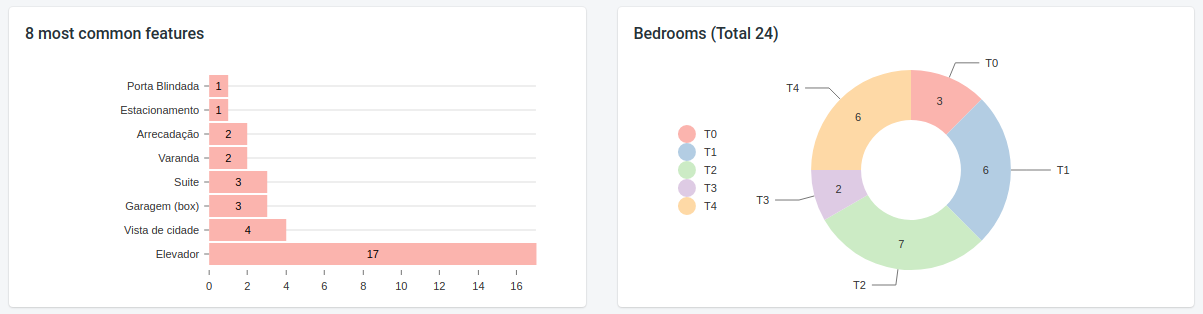
\includegraphics[width=1\linewidth]{Chapters/img/frontend/OverviewEstateData.png}
	\caption{Information about the estates in the zone}
	\label{fig:overviewSearchBar}
\end{figure}

\paragraph{Estates} is the most important section of the dashboard, right after the map, as it allows the user to browse each estate and see his personalized index associated with each estate. The table allows the user to select the number of estates to display per page, sort the estates by the numerous fields, numerically or alphabetically, while also allowing the user to filter results by pressing the header and entering out their queries (e..g., price > 10).

\begin{figure}[h]
	\centering
	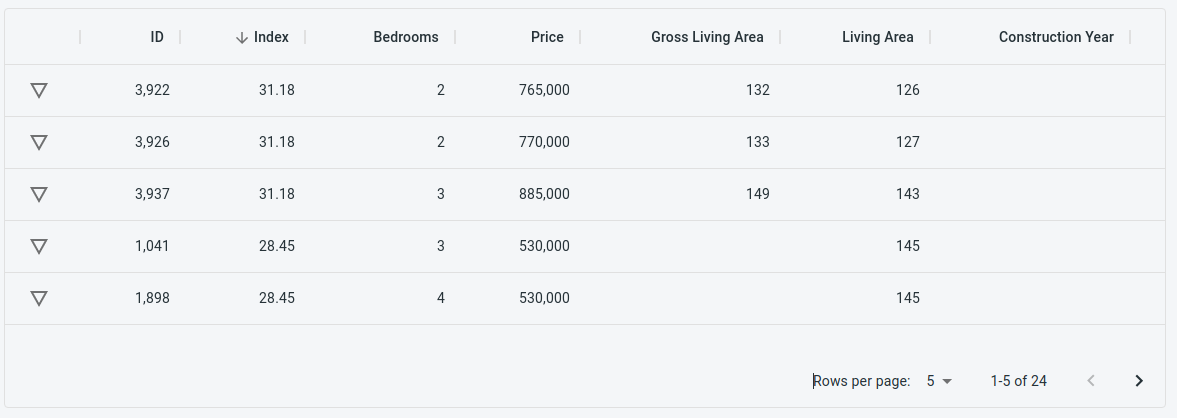
\includegraphics[width=1\linewidth]{Chapters/img/frontend/OverviewEstateListIndex.png}
	\caption{List of estates in the selected zone}
	\label{fig:overviewListEstate}
\end{figure}

Additionally, each row is accompanied by a triangle, this symbol represents the ability to expand each estate and learn more about it.

\begin{figure}[h]
	\centering
	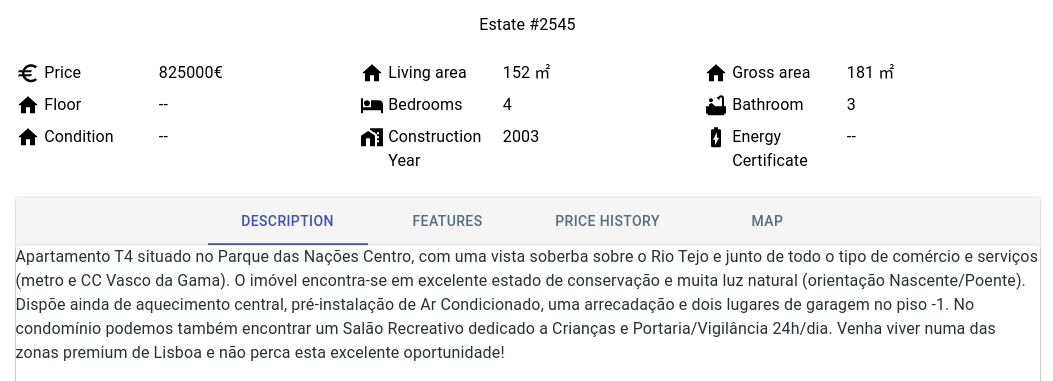
\includegraphics[width=1\linewidth]{Chapters/img/frontend/DetailedDescription.png}
	\caption{Estate list data}
	\label{fig:detailed}
\end{figure}

In this modal (window popup), the user can read the original description extracted during the scraping, the features associated with each estate, the price history with the scraped price after each iteration, and the location of the estate in the map, but unlike the previous map the zone shown actually represents the area the user can reach with the selected travel mode in 15 minutes, along with all containing points of interest (even the ones that do not belong to the current selected zone). 

\begin{figure}[H]
    \centering
    \begin{subfigure}[b]{0.49\textwidth}
        \centering
        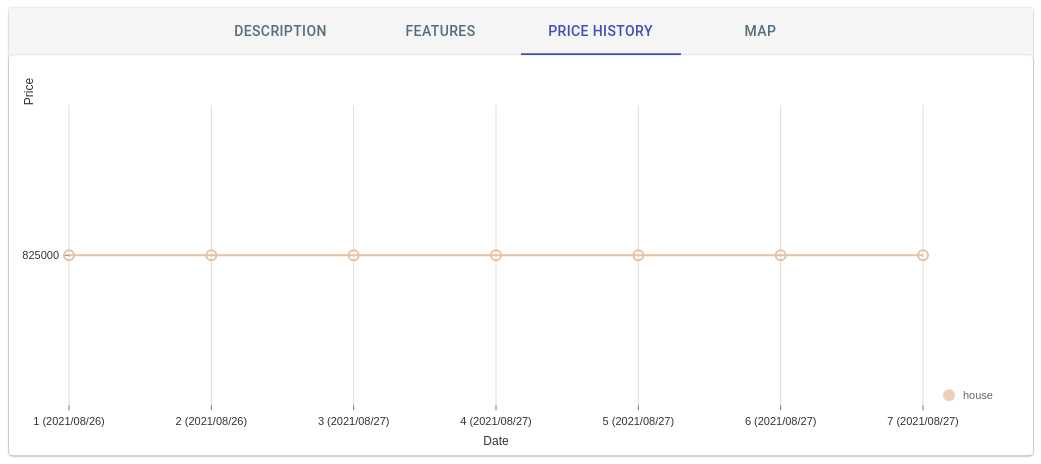
\includegraphics[width=1\linewidth]{Chapters/img/frontend/DetailedPriceHistory.png}
        \caption{u}
        \label{fig:detailedPriceHistory}
     \end{subfigure}
     \hfill
     \begin{subfigure}[b]{0.49\textwidth}
        \centering
        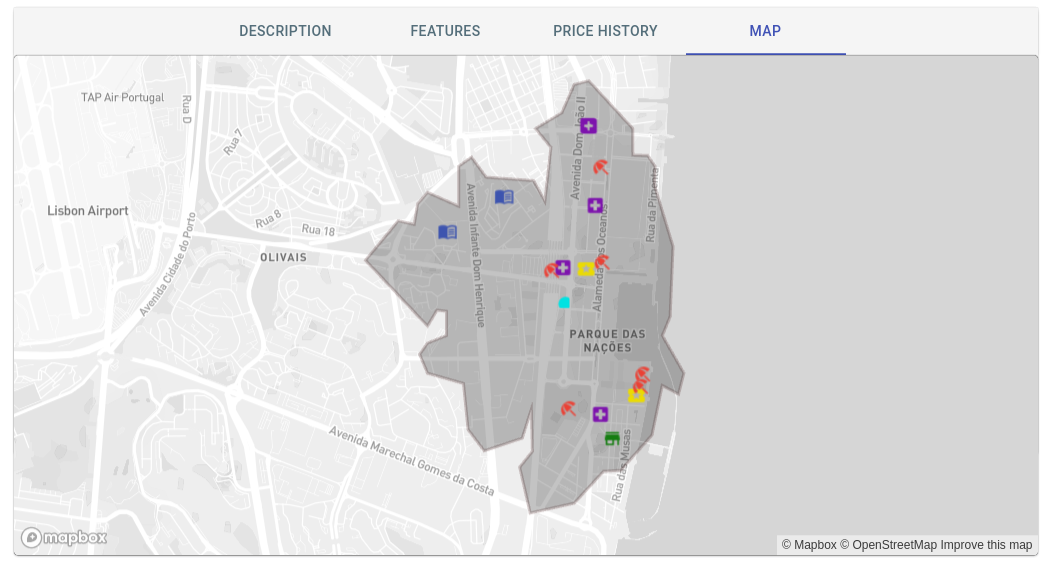
\includegraphics[width=1\linewidth]{Chapters/img/frontend/DetailedIsochrone.png}
        \caption{r}
        \label{fig:detailedIsochrone}
     \end{subfigure}
     \caption{Tabs of detailed view}
\end{figure}

